\subsection{Determinação da capacidade térmica do calorímetro}

Nesse primeiro experimento, iremos determinar a capacidade térmica $C$ do nosso calorímetro - aparelho que será importante para os demais experimentos.\\

De início, vamos explicar melhor o funcionamento de um calorímetro. Ao longo dos experimentos, iremos considerá-lo como um sistema termicamente isolado, no qual não irão acontecer trocas de calor entre o interior do calorímetro e o meio externo. Se uma quantidade $N$ de corpos, todos com temperaturas diferentes, forem inseridos em um calorímetro, eles trocarão calor entre si até atingirem uma temperatura comum, de tal forma, a soma algébrica das quantidades de calor $\Delta Q_i$ trocadas até que o equilíbrio térmico ocorra, será zero:
\[ \sum_{i=1}^{N} Q_i = 0\]

Esse fato ocorre, pois consideramos o sistema como isolado, e a energia total desse tipo de sistema é constante.\\

Para estudar melhor as trocas de calor - já explicadas anteriormente - colocaremos as substancias ou os corpos no interior de calorímetros, que isolarão termicamente as nossas amostras do meio externo, permitindo uma melhor análise. Como geralmente um calorímetro não é formado por um único material - não podendo assumir um calor específico exato para ele - e, também, contém partes que participam das trocas de calor que estão ocorrendo em seu interior - fazendo com que ele próprio mude de temperatura -, definimos a capacidade térmica $C$ do calorímetro. Esse valor encontrado permite que relacionemos a quantidade de calor envolvida na variação de temperatura experimentada pelo calorímetro, do seguinte modo:
\[ Q = C \Delta T\]

\begin{figure}[H]
  \centering
  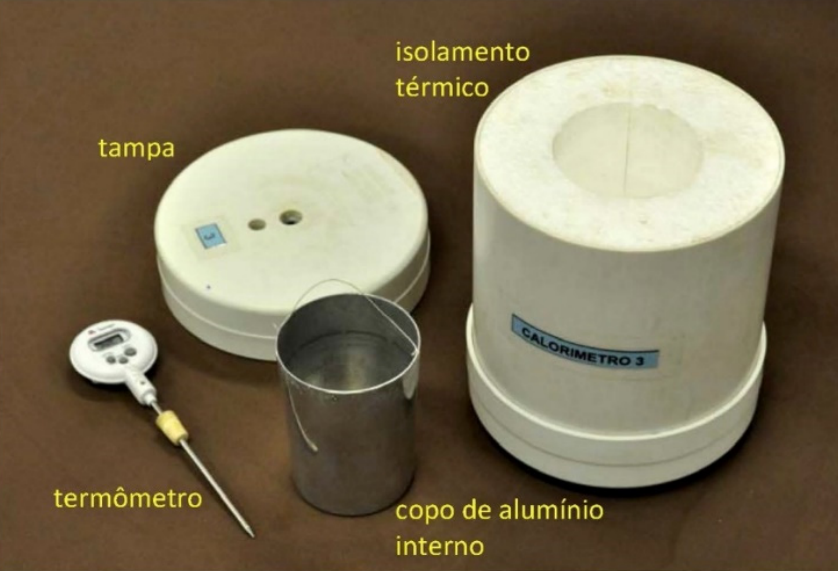
\includegraphics[scale=0.67]{images/calorimetro.png}
  \caption{Foto do calorímetro utilizado em nossos experimentos.}
\end{figure}

Desse modo, podemos iniciar a explicação do nosso experimento inicial.\\

Para determinar a capacidade térmica do calorímetro, vamos considerar uma quantidade de água de massa $m_1$, que está a uma temperatura inicial $T_1$, em equilíbrio com o calorímetro. Vamos colocar uma segunda quantidade de água de massa $m_2$ a uma temperatura $T_2$ no interior do calorímetro (sabemos que $T_2 > T_1$).\\

Caso o calorímetro fosse ideal, com capacidade térmica nula ($C$ = 0), a transferência de calor entre essas quantidades de água seria apenas da porção mais quente para a porção mais fria, e essa relação seria dada por:
\[m_1 c_a(T_f - T_1) + m_2 c_a(T_f - T_2) = 0 \]
em que $T_f$ é a temperatura final de equilíbrio do sistema, intermediária às outras duas ( $T_2 > T_f > T_1$ ) e $c_a$ é o calor específico da água.\\

Porém, no nosso caso, tratamos de um calorímetro real, no qual haverá troca de calor entre ele a as substâncias nele contidas. Assim, devemos adicionar essa quantidade de calor trocada à nossa equação, obtendo: 
\[m_1 c_a(T_f - T_1) + m_2 c_a(T_f - T_2) + C (T_f - T_1) = 0 \]
Se isolarmos a capacidade térmica, chegaremos à uma equação que calcula $C$ em função das temperaturas, massas e calores específicos envolvidos no problema:
\[C =  \frac{m_2 c_a (T_2 - T_f) }{(T_f - T_1)} - m_1 c_a \]

OBS: A unidade usada no SI é J/K (Joule por Kelvin). Por motivos históricos, é comum o uso da unidade caloria por graus Celsius (cal/°C), que será usada por nós em nossos experimentos.\\

Esse é o experimento inicial, no qual vamos deduzir a capacidade térmica do nosso calorímetro pela fórmula acima.
